\documentclass{standalone}

%\usepackage[a2paper]{geometry}
\usepackage[utf8]{inputenc}
\usepackage{braket}									%Dirac Schreibweise
\usepackage{tikz}
\usetikzlibrary{arrows,positioning,shapes,backgrounds,fit}  
\usetikzlibrary{decorations.text}
\usetikzlibrary{decorations}
\usetikzlibrary{%
    decorations.pathreplacing,%
    decorations.pathmorphing%
}
\usepackage{pgfplots}
\pgfplotsset{width=8cm,compat=1.8}

\usepackage{amsmath}
\usepackage{xcolor}
\definecolor{DarkBlue}{rgb}{0.1,0.1,0.5}
\definecolor{Blue}{rgb}{0.1,0.1,0.8}
\definecolor{Red}{rgb}{0.75,0.,0.}
\definecolor{Gray}{gray}{0.3}
\definecolor{Green}{rgb}{0.2,0.5,0.2}
\newcommand*\circled[1]{\tikz[baseline=(char.base)]{\node[shape=circle,draw,inner sep=2pt] (char) {#1};}}



\begin{document}
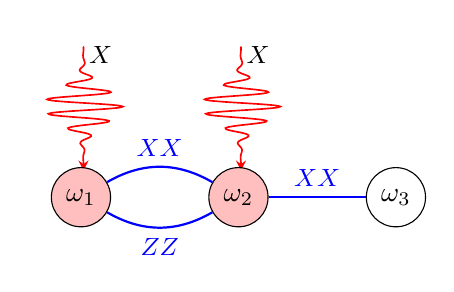
\begin{tikzpicture}

%% C12

% First pulse
\node[rotate=-90] at (0.05,1.1)
    (pulse) {% 
    \tikz{% 
    \node[align=center] at (0.0,2.5) {%
    \tikz[xscale=0.6]{% 
    \draw[% 
 red,thick, xscale=0.5, yscale=0.5, domain=2.5:7.5, smooth, variable=\x, samples=100, anchor=center, line cap=round, -stealth, shorten >=-2pt, line width=0.6pt ] plot ({\x},{exp(-(\x-5)*(\x-5))*(cos(10*\x r))}); } }; } };
    \node[](q1) at (0.25,1.8){\small $X$};

% Second pulse
\node[rotate=-90] at (2.05,1.1)
    (pulse) {% 
    \tikz{% 
    \node[align=center] at (2.0,2.5) {%
    \tikz[xscale=0.6]{% 
    \draw[% 
 red,thick, xscale=0.5, yscale=0.5, domain=2.5:7.5, smooth, variable=\x, samples=100, anchor=center, line cap=round, -stealth, shorten >=-2pt, line width=0.6pt ] plot ({\x},{exp(-(\x-5)*(\x-5))*(cos(10*\x r))}); } }; } };
    \node[](q2) at (2.25,1.8){\small $X$};

    

\node[circle, draw = black,fill=pink](p1) at (0,0){$\omega_{1}$};
\node[circle, draw = black,fill=pink](p2) at (2,0){$\omega_{2}$};
\node[circle, draw = black](p3) at (4,0){$\omega_{3}$};



\path[every node/.style={sloped,anchor=south,auto=false}]
(p1) edge[blue, bend left=30,thick]  node  {\small $XX$} (p2);


\path[every node/.style={sloped,anchor=south,auto=false}](p1) edge[blue, bend right=30,thick]  node [below]   {\small $ZZ$} (p2);

\path[every node/.style={sloped,anchor=south,auto=false}]
(p2)edge[blue,thick] node {\small ${XX}$} (p3);



\end{tikzpicture}
\end{document}